\documentclass[12pt,a4paper]{article}

\usepackage[a4paper,text={16.5cm,25.2cm},centering]{geometry}
\usepackage{lmodern}
\usepackage{amssymb,amsmath}
\usepackage{bm}
\usepackage{graphicx}
\usepackage{microtype}
\usepackage{hyperref}
\setlength{\parindent}{0pt}
\setlength{\parskip}{1.2ex}

\hypersetup
       {   pdfauthor = { Sheehan Olver },
           pdftitle={ foo },
           colorlinks=TRUE,
           linkcolor=black,
           citecolor=blue,
           urlcolor=blue
       }




\usepackage{upquote}
\usepackage{listings}
\usepackage{xcolor}
\lstset{
    basicstyle=\ttfamily\footnotesize,
    upquote=true,
    breaklines=true,
    breakindent=0pt,
    keepspaces=true,
    showspaces=false,
    columns=fullflexible,
    showtabs=false,
    showstringspaces=false,
    escapeinside={(*@}{@*)},
    extendedchars=true,
}
\newcommand{\HLJLt}[1]{#1}
\newcommand{\HLJLw}[1]{#1}
\newcommand{\HLJLe}[1]{#1}
\newcommand{\HLJLeB}[1]{#1}
\newcommand{\HLJLo}[1]{#1}
\newcommand{\HLJLk}[1]{\textcolor[RGB]{148,91,176}{\textbf{#1}}}
\newcommand{\HLJLkc}[1]{\textcolor[RGB]{59,151,46}{\textit{#1}}}
\newcommand{\HLJLkd}[1]{\textcolor[RGB]{214,102,97}{\textit{#1}}}
\newcommand{\HLJLkn}[1]{\textcolor[RGB]{148,91,176}{\textbf{#1}}}
\newcommand{\HLJLkp}[1]{\textcolor[RGB]{148,91,176}{\textbf{#1}}}
\newcommand{\HLJLkr}[1]{\textcolor[RGB]{148,91,176}{\textbf{#1}}}
\newcommand{\HLJLkt}[1]{\textcolor[RGB]{148,91,176}{\textbf{#1}}}
\newcommand{\HLJLn}[1]{#1}
\newcommand{\HLJLna}[1]{#1}
\newcommand{\HLJLnb}[1]{#1}
\newcommand{\HLJLnbp}[1]{#1}
\newcommand{\HLJLnc}[1]{#1}
\newcommand{\HLJLncB}[1]{#1}
\newcommand{\HLJLnd}[1]{\textcolor[RGB]{214,102,97}{#1}}
\newcommand{\HLJLne}[1]{#1}
\newcommand{\HLJLneB}[1]{#1}
\newcommand{\HLJLnf}[1]{\textcolor[RGB]{66,102,213}{#1}}
\newcommand{\HLJLnfm}[1]{\textcolor[RGB]{66,102,213}{#1}}
\newcommand{\HLJLnp}[1]{#1}
\newcommand{\HLJLnl}[1]{#1}
\newcommand{\HLJLnn}[1]{#1}
\newcommand{\HLJLno}[1]{#1}
\newcommand{\HLJLnt}[1]{#1}
\newcommand{\HLJLnv}[1]{#1}
\newcommand{\HLJLnvc}[1]{#1}
\newcommand{\HLJLnvg}[1]{#1}
\newcommand{\HLJLnvi}[1]{#1}
\newcommand{\HLJLnvm}[1]{#1}
\newcommand{\HLJLl}[1]{#1}
\newcommand{\HLJLld}[1]{\textcolor[RGB]{148,91,176}{\textit{#1}}}
\newcommand{\HLJLs}[1]{\textcolor[RGB]{201,61,57}{#1}}
\newcommand{\HLJLsa}[1]{\textcolor[RGB]{201,61,57}{#1}}
\newcommand{\HLJLsb}[1]{\textcolor[RGB]{201,61,57}{#1}}
\newcommand{\HLJLsc}[1]{\textcolor[RGB]{201,61,57}{#1}}
\newcommand{\HLJLsd}[1]{\textcolor[RGB]{201,61,57}{#1}}
\newcommand{\HLJLsdB}[1]{\textcolor[RGB]{201,61,57}{#1}}
\newcommand{\HLJLsdC}[1]{\textcolor[RGB]{201,61,57}{#1}}
\newcommand{\HLJLse}[1]{\textcolor[RGB]{59,151,46}{#1}}
\newcommand{\HLJLsh}[1]{\textcolor[RGB]{201,61,57}{#1}}
\newcommand{\HLJLsi}[1]{#1}
\newcommand{\HLJLso}[1]{\textcolor[RGB]{201,61,57}{#1}}
\newcommand{\HLJLsr}[1]{\textcolor[RGB]{201,61,57}{#1}}
\newcommand{\HLJLss}[1]{\textcolor[RGB]{201,61,57}{#1}}
\newcommand{\HLJLssB}[1]{\textcolor[RGB]{201,61,57}{#1}}
\newcommand{\HLJLnB}[1]{\textcolor[RGB]{59,151,46}{#1}}
\newcommand{\HLJLnbB}[1]{\textcolor[RGB]{59,151,46}{#1}}
\newcommand{\HLJLnfB}[1]{\textcolor[RGB]{59,151,46}{#1}}
\newcommand{\HLJLnh}[1]{\textcolor[RGB]{59,151,46}{#1}}
\newcommand{\HLJLni}[1]{\textcolor[RGB]{59,151,46}{#1}}
\newcommand{\HLJLnil}[1]{\textcolor[RGB]{59,151,46}{#1}}
\newcommand{\HLJLnoB}[1]{\textcolor[RGB]{59,151,46}{#1}}
\newcommand{\HLJLoB}[1]{\textcolor[RGB]{102,102,102}{\textbf{#1}}}
\newcommand{\HLJLow}[1]{\textcolor[RGB]{102,102,102}{\textbf{#1}}}
\newcommand{\HLJLp}[1]{#1}
\newcommand{\HLJLc}[1]{\textcolor[RGB]{153,153,119}{\textit{#1}}}
\newcommand{\HLJLch}[1]{\textcolor[RGB]{153,153,119}{\textit{#1}}}
\newcommand{\HLJLcm}[1]{\textcolor[RGB]{153,153,119}{\textit{#1}}}
\newcommand{\HLJLcp}[1]{\textcolor[RGB]{153,153,119}{\textit{#1}}}
\newcommand{\HLJLcpB}[1]{\textcolor[RGB]{153,153,119}{\textit{#1}}}
\newcommand{\HLJLcs}[1]{\textcolor[RGB]{153,153,119}{\textit{#1}}}
\newcommand{\HLJLcsB}[1]{\textcolor[RGB]{153,153,119}{\textit{#1}}}
\newcommand{\HLJLg}[1]{#1}
\newcommand{\HLJLgd}[1]{#1}
\newcommand{\HLJLge}[1]{#1}
\newcommand{\HLJLgeB}[1]{#1}
\newcommand{\HLJLgh}[1]{#1}
\newcommand{\HLJLgi}[1]{#1}
\newcommand{\HLJLgo}[1]{#1}
\newcommand{\HLJLgp}[1]{#1}
\newcommand{\HLJLgs}[1]{#1}
\newcommand{\HLJLgsB}[1]{#1}
\newcommand{\HLJLgt}[1]{#1}



\def\qqand{\qquad\hbox{and}\qquad}
\def\qqfor{\qquad\hbox{for}\qquad}
\def\qqas{\qquad\hbox{as}\qquad}
\def\D{ {\rm d} }
\def\I{ {\rm i} }
\def\E{ {\rm e} }
\def\C{ {\mathbb C} }
\def\R{ {\mathbb R} }
\def\CC{ {\cal C} }
\def\HH{ {\cal H} }
\def\LL{ {\cal L} }
\def\vc#1{ {\mathbf #1} }
\def\bbC{ {\mathbb C} }

\def\qqqquad{\qquad\qquad}
\def\qqwhere{\qquad\hbox{where}\qquad}
\def\Res_#1{\underset{#1}{\rm Res}\,}
\def\sech{ {\rm sech}\, }
\def\acos{ {\rm acos}\, }
\def\atan{ {\rm atan}\, }
\def\upepsilon{\varepsilon}


\def\Xint#1{ \mathchoice
   {\XXint\displaystyle\textstyle{#1} }%
   {\XXint\textstyle\scriptstyle{#1} }%
   {\XXint\scriptstyle\scriptscriptstyle{#1} }%
   {\XXint\scriptscriptstyle\scriptscriptstyle{#1} }%
   \!\int}
\def\XXint#1#2#3{ {\setbox0=\hbox{$#1{#2#3}{\int}$}
     \vcenter{\hbox{$#2#3$}}\kern-.5\wd0} }
\def\ddashint{\Xint=}
\def\dashint{\Xint-}
% \def\dashint
\def\infdashint{\dashint_{-\infty}^\infty}




\def\addtab#1={#1\;&=}
\def\ccr{\\\addtab}
\def\ip<#1>{\left\langle{#1}\right\rangle}
\def\dx{\D x}
\def\dt{\D t}
\def\dz{\D z}

\def\norm#1{\left\| #1 \right\|}

\def\pr(#1){\left({#1}\right)}
\def\br[#1]{\left[{#1}\right]}

\def\abs#1{\left|{#1}\right|}
\def\fpr(#1){\!\pr({#1})}

\def\sopmatrix#1{ \begin{pmatrix}#1\end{pmatrix} }

\def\endash{–}
\def\mdblksquare{\blacksquare}
\def\lgblksquare{\blacksquare}
\def\scre{\E}
\def\mapengine#1,#2.{\mapfunction{#1}\ifx\void#2\else\mapengine #2.\fi }

\def\map[#1]{\mapengine #1,\void.}

\def\mapenginesep_#1#2,#3.{\mapfunction{#2}\ifx\void#3\else#1\mapengine #3.\fi }

\def\mapsep_#1[#2]{\mapenginesep_{#1}#2,\void.}


\def\vcbr[#1]{\pr(#1)}


\def\bvect[#1,#2]{
{
\def\dots{\cdots}
\def\mapfunction##1{\ | \  ##1}
	\sopmatrix{
		 \,#1\map[#2]\,
	}
}
}



\def\vect[#1]{
{\def\dots{\ldots}
	\vcbr[{#1}]
} }

\def\vectt[#1]{
{\def\dots{\ldots}
	\vect[{#1}]^{\top}
} }

\def\Vectt[#1]{
{
\def\mapfunction##1{##1 \cr} 
\def\dots{\vdots}
	\begin{pmatrix}
		\map[#1]
	\end{pmatrix}
} }

\def\addtab#1={#1\;&=}
\def\ccr{\\\addtab}

\begin{document}

\textbf{M3M6: Methods of Mathematical Physics}

Dr. Sheehan Olver

s.olver@imperial.ac.uk

\section{Inverting Log kernels}
\begin{itemize}
\item[2. ] Solving a logarithmic singular integral equation


\item[3. ] Application: electrostatic potentials in 2D

\begin{itemize}
\item Potential arising from a point charge and a single plate

\end{itemize}
\end{itemize}
\subsubsection{Solving logarithmic singular integral equations}
Consider the problem of calculating $u(x)$ such that

\[
{1 \over \pi} \int_a^b u(t) \log | x-t| \dt = f(x) \qqfor a < x < b
\]
To tackle this problem, recall that $L u(z) = \Re M u(z)$ for

\[
M u(z) = {1 \over \pi} \int_a^b \log|z-t| u(t) \D t =  -2 \I \int_c^z \CC u(\zeta) \D \zeta + M u(c)
\]
where $c$ is arbitrary, in fact we can choose it to be $b$. Then we have

\[
L u(x) =  \Re M^+ u(x) = 2\Im \int_b^x \CC^+ u(t) \D t =  \int_b^x H u(t) \D t
\]
where 

\[
\HH u(x) = {1 \over \pi} \dashint_a^b {u(t) \over t -x } \D t
\]
is the Hilbert transform. In other words, we have

\[
{\D \over \dx} L u(x) = \HH u(x).
\]
Differentiating both sides of the equation for $u$ therefore gives

\[
\HH u(x) = f'(x).
\]
recall, we can express the solution as

\[
    u = {-\HH[\sqrt{b-\diamond}\sqrt{\diamond-a} f'] + D \over \sqrt{b-x}\sqrt{x-a}} 
\]
Here the constant $D$ is not arbitrary: recall that

\[
\LL[1/\sqrt{1-\diamond^2}](x) = - \log 2
\]
hence varying $D$ will vary $u$ by a constant. To choose $D$,  we use the fact that

\[
f(c) = {1 \over \pi} \int_a^b u(t) \log |t-c| \dt
\]
for any choice of point  $c$.

\textbf{Demonstration}

Let's do a numerical example:


\begin{lstlisting}
(*@\HLJLk{using}@*) (*@\HLJLn{ApproxFun}@*)(*@\HLJLp{,}@*) (*@\HLJLn{SingularIntegralEquations}@*)(*@\HLJLp{,}@*) (*@\HLJLn{Plots}@*)
(*@\HLJLnf{H}@*)(*@\HLJLp{(}@*)(*@\HLJLn{f}@*)(*@\HLJLp{)}@*) (*@\HLJLoB{=}@*) (*@\HLJLoB{-}@*)(*@\HLJLnf{hilbert}@*)(*@\HLJLp{(}@*)(*@\HLJLn{f}@*)(*@\HLJLp{)}@*) (*@\HLJLcs{{\#}}@*) (*@\HLJLcs{fix}@*) (*@\HLJLcs{normalisation}@*)
(*@\HLJLnf{H}@*)(*@\HLJLp{(}@*)(*@\HLJLn{f}@*)(*@\HLJLp{,}@*)(*@\HLJLn{x}@*)(*@\HLJLp{)}@*) (*@\HLJLoB{=}@*) (*@\HLJLoB{-}@*)(*@\HLJLnf{hilbert}@*)(*@\HLJLp{(}@*)(*@\HLJLn{f}@*)(*@\HLJLp{,}@*)(*@\HLJLn{x}@*)(*@\HLJLp{)}@*)


(*@\HLJLn{x}@*) (*@\HLJLoB{=}@*) (*@\HLJLnf{Fun}@*)(*@\HLJLp{()}@*)
(*@\HLJLn{f}@*) (*@\HLJLoB{=}@*) (*@\HLJLnf{exp}@*)(*@\HLJLp{(}@*)(*@\HLJLn{x}@*)(*@\HLJLp{)}@*)
(*@\HLJLn{D}@*) (*@\HLJLoB{=}@*) (*@\HLJLnf{randn}@*)(*@\HLJLp{()}@*)

(*@\HLJLn{u\ensuremath{\_1}}@*) (*@\HLJLoB{=}@*) (*@\HLJLoB{-}@*)(*@\HLJLnf{H}@*)(*@\HLJLp{(}@*)(*@\HLJLnf{sqrt}@*)(*@\HLJLp{(}@*)(*@\HLJLni{1}@*)(*@\HLJLoB{-}@*)(*@\HLJLn{x}@*)(*@\HLJLoB{{\textasciicircum}}@*)(*@\HLJLni{2}@*)(*@\HLJLp{)}@*)(*@\HLJLoB{*}@*)(*@\HLJLn{f}@*)(*@\HLJLoB{{\textquotesingle}}@*)(*@\HLJLp{)}@*)(*@\HLJLoB{/}@*)(*@\HLJLnf{sqrt}@*)(*@\HLJLp{(}@*)(*@\HLJLni{1}@*)(*@\HLJLoB{-}@*)(*@\HLJLn{x}@*)(*@\HLJLoB{{\textasciicircum}}@*)(*@\HLJLni{2}@*)(*@\HLJLp{)}@*) 

(*@\HLJLn{u}@*) (*@\HLJLoB{=}@*) (*@\HLJLn{u\ensuremath{\_1}}@*) (*@\HLJLoB{+}@*) (*@\HLJLn{D}@*)(*@\HLJLoB{/}@*)(*@\HLJLnf{sqrt}@*)(*@\HLJLp{(}@*)(*@\HLJLni{1}@*)(*@\HLJLoB{-}@*)(*@\HLJLn{x}@*)(*@\HLJLoB{{\textasciicircum}}@*)(*@\HLJLni{2}@*)(*@\HLJLp{)}@*)

(*@\HLJLnd{@show}@*) (*@\HLJLnf{H}@*)(*@\HLJLp{(}@*)(*@\HLJLn{u}@*)(*@\HLJLp{,}@*) (*@\HLJLnfB{0.1}@*)(*@\HLJLp{)}@*) (*@\HLJLoB{+}@*) (*@\HLJLnf{f}@*)(*@\HLJLp{(}@*)(*@\HLJLnfB{0.1}@*)(*@\HLJLp{)}@*)
\end{lstlisting}

\begin{lstlisting}
H(u, 0.1) + f(0.1) = 2.2103418361512954
\end{lstlisting}


\begin{lstlisting}
(*@\HLJLnd{@show}@*) (*@\HLJLnf{logkernel}@*)(*@\HLJLp{(}@*)(*@\HLJLn{u}@*)(*@\HLJLp{,}@*)(*@\HLJLnfB{0.1}@*)(*@\HLJLp{)}@*) (*@\HLJLoB{-}@*) (*@\HLJLnf{f}@*)(*@\HLJLp{(}@*)(*@\HLJLnfB{0.1}@*)(*@\HLJLp{)}@*)  (*@\HLJLcs{{\#}}@*) (*@\HLJLcs{didn{\textquotesingle}t}@*) (*@\HLJLcs{work}@*)
\end{lstlisting}

\begin{lstlisting}
logkernel(u, 0.1) - f(0.1) = -0.0941709295301647
\end{lstlisting}


\begin{lstlisting}
(*@\HLJLnd{@show}@*) (*@\HLJLnf{logkernel}@*)(*@\HLJLp{(}@*)(*@\HLJLn{u}@*)(*@\HLJLp{,}@*)(*@\HLJLnfB{0.2}@*)(*@\HLJLp{)}@*) (*@\HLJLoB{-}@*) (*@\HLJLnf{f}@*)(*@\HLJLp{(}@*)(*@\HLJLnfB{0.2}@*)(*@\HLJLp{);}@*)  (*@\HLJLcs{{\#}}@*) (*@\HLJLcs{but}@*) (*@\HLJLcs{we}@*) (*@\HLJLcs{are}@*) (*@\HLJLcs{only}@*) (*@\HLJLcs{off}@*) (*@\HLJLcs{by}@*) (*@\HLJLcs{a}@*) (*@\HLJLcs{constant}@*)
\end{lstlisting}

\begin{lstlisting}
logkernel(u, 0.2) - f(0.2) = -0.09417092953016448
\end{lstlisting}


We thus need to choose the constant


\begin{lstlisting}
(*@\HLJLcs{{\#}}@*) (*@\HLJLcs{choose}@*) (*@\HLJLcs{C}@*) (*@\HLJLcs{so}@*) (*@\HLJLcs{that}@*)
(*@\HLJLcs{{\#}}@*) (*@\HLJLcs{logkernel(u\ensuremath{\_1},}@*) (*@\HLJLcs{0)}@*) (*@\HLJLcs{+}@*) (*@\HLJLcs{C*logkernel(1/sqrt(1-x{\textasciicircum}2),}@*) (*@\HLJLcs{0)}@*) (*@\HLJLcs{==}@*) (*@\HLJLcs{f(0)}@*)
(*@\HLJLn{C}@*) (*@\HLJLoB{=}@*) (*@\HLJLp{(}@*)(*@\HLJLnf{f}@*)(*@\HLJLp{(}@*)(*@\HLJLni{0}@*)(*@\HLJLp{)}@*) (*@\HLJLoB{-}@*) (*@\HLJLnf{logkernel}@*)(*@\HLJLp{(}@*)(*@\HLJLn{u\ensuremath{\_1}}@*)(*@\HLJLp{,}@*) (*@\HLJLni{0}@*)(*@\HLJLp{))}@*)(*@\HLJLoB{/}@*)(*@\HLJLnf{logkernel}@*)(*@\HLJLp{(}@*)(*@\HLJLni{1}@*)(*@\HLJLoB{/}@*)(*@\HLJLnf{sqrt}@*)(*@\HLJLp{(}@*)(*@\HLJLni{1}@*)(*@\HLJLoB{-}@*)(*@\HLJLn{x}@*)(*@\HLJLoB{{\textasciicircum}}@*)(*@\HLJLni{2}@*)(*@\HLJLp{),}@*) (*@\HLJLni{0}@*)(*@\HLJLp{)}@*)
(*@\HLJLn{u}@*) (*@\HLJLoB{=}@*) (*@\HLJLn{u\ensuremath{\_1}}@*) (*@\HLJLoB{+}@*) (*@\HLJLn{C}@*)(*@\HLJLoB{/}@*)(*@\HLJLnf{sqrt}@*)(*@\HLJLp{(}@*)(*@\HLJLni{1}@*)(*@\HLJLoB{-}@*)(*@\HLJLn{x}@*)(*@\HLJLoB{{\textasciicircum}}@*)(*@\HLJLni{2}@*)(*@\HLJLp{)}@*)

(*@\HLJLnd{@show}@*) (*@\HLJLnf{hilbert}@*)(*@\HLJLp{(}@*)(*@\HLJLn{u}@*)(*@\HLJLp{,}@*) (*@\HLJLnfB{0.1}@*)(*@\HLJLp{)}@*) (*@\HLJLoB{+}@*) (*@\HLJLnf{f}@*)(*@\HLJLp{(}@*)(*@\HLJLnfB{0.1}@*)(*@\HLJLp{)}@*)
\end{lstlisting}

\begin{lstlisting}
hilbert(u, 0.1) + f(0.1) = -6.661338147750939e-16
\end{lstlisting}


\begin{lstlisting}
(*@\HLJLnd{@show}@*) (*@\HLJLnf{logkernel}@*)(*@\HLJLp{(}@*)(*@\HLJLn{u}@*)(*@\HLJLp{,}@*)(*@\HLJLnfB{0.1}@*)(*@\HLJLp{)}@*) (*@\HLJLoB{-}@*) (*@\HLJLnf{f}@*)(*@\HLJLp{(}@*)(*@\HLJLnfB{0.1}@*)(*@\HLJLp{)}@*)  (*@\HLJLcs{{\#}}@*) (*@\HLJLcs{Works!}@*)
\end{lstlisting}

\begin{lstlisting}
logkernel(u, 0.1) - f(0.1) = -2.220446049250313e-16
\end{lstlisting}


\begin{lstlisting}
(*@\HLJLnd{@show}@*) (*@\HLJLnf{logkernel}@*)(*@\HLJLp{(}@*)(*@\HLJLn{u}@*)(*@\HLJLp{,}@*)(*@\HLJLnfB{0.2}@*)(*@\HLJLp{)}@*) (*@\HLJLoB{-}@*) (*@\HLJLnf{f}@*)(*@\HLJLp{(}@*)(*@\HLJLnfB{0.2}@*)(*@\HLJLp{);}@*)  (*@\HLJLcs{{\#}}@*) (*@\HLJLcs{And}@*) (*@\HLJLcs{at}@*) (*@\HLJLcs{all}@*) (*@\HLJLcs{x!}@*)
\end{lstlisting}

\begin{lstlisting}
logkernel(u, 0.2) - f(0.2) = 0.0
\end{lstlisting}


\textbf{Example 1} We now do an example which can be solved by hand.  Find $u(x)$ so that: 

\[
\LL u(x) = x
\]
for $-1 < x < 1$. Differentiating his becomes

\[
\HH u(x) = 1
\]
which we solve via

\[
u(x) = {- \HH[\sqrt{1-\diamond^2}](x) + D \over \sqrt{1-x^2}} = {D-x \over \sqrt{1-x^2}}
\]
Note that 

\[
\LL u(0) = 0
\]
A symmetry argument shows that

\[
\LL [\diamond/\sqrt{1-\diamond^2}](x) = {1 \over \pi} \int_{-1}^1 {x \over \sqrt{1-x^2}} \log|x| \D x = 0
\]
which imples that $D = 0$ and we have 

\[
u(x) = {-x \over \sqrt{1-x^2}}
\]
We can confirm this:


\begin{lstlisting}
(*@\HLJLn{x}@*) (*@\HLJLoB{=}@*) (*@\HLJLnf{Fun}@*)(*@\HLJLp{()}@*)
(*@\HLJLnf{logkernel}@*)(*@\HLJLp{(}@*)(*@\HLJLoB{-}@*)(*@\HLJLn{x}@*)(*@\HLJLoB{/}@*)(*@\HLJLnf{sqrt}@*)(*@\HLJLp{(}@*)(*@\HLJLni{1}@*)(*@\HLJLoB{-}@*)(*@\HLJLn{x}@*)(*@\HLJLoB{{\textasciicircum}}@*)(*@\HLJLni{2}@*)(*@\HLJLp{),}@*) (*@\HLJLnfB{0.1}@*)(*@\HLJLp{)}@*) (*@\HLJLcs{{\#}}@*) (*@\HLJLcs{approximately}@*) (*@\HLJLcs{0.1}@*)
\end{lstlisting}

\begin{lstlisting}
0.10000000000000006
\end{lstlisting}


\textbf{Example 2} Find $u(x)$ so that: 

\[
{1 \over \pi} \int_{-1}^1 u(t) \log | x-t| \dt = 1.
\]
Differentiating, we know that 

\[
\int_{-1}^1 {u(t) \over x-t} \dt = 0
\]
hence $u(x)$ must be of the form ${D / \sqrt{1-x^2}}$.  Since we know 

\[
\L[{1 /\sqrt{1-\diamond^2}}](x) = - \log 2
\]
we have $D = -1/\log 2$. Let's check:


\begin{lstlisting}
(*@\HLJLn{x}@*) (*@\HLJLoB{=}@*) (*@\HLJLnf{Fun}@*)(*@\HLJLp{()}@*)
(*@\HLJLn{u}@*) (*@\HLJLoB{=}@*) (*@\HLJLoB{-}@*)(*@\HLJLni{1}@*)(*@\HLJLoB{/}@*)(*@\HLJLp{(}@*)(*@\HLJLnf{log}@*)(*@\HLJLp{(}@*)(*@\HLJLni{2}@*)(*@\HLJLp{)}@*)(*@\HLJLoB{*}@*)(*@\HLJLnf{sqrt}@*)(*@\HLJLp{(}@*)(*@\HLJLni{1}@*)(*@\HLJLoB{-}@*)(*@\HLJLn{x}@*)(*@\HLJLoB{{\textasciicircum}}@*)(*@\HLJLni{2}@*)(*@\HLJLp{))}@*)
(*@\HLJLnf{logkernel}@*)(*@\HLJLp{(}@*)(*@\HLJLn{u}@*)(*@\HLJLp{,}@*) (*@\HLJLnfB{0.1}@*)(*@\HLJLp{)}@*) (*@\HLJLcs{{\#}}@*) (*@\HLJLcs{approximately}@*) (*@\HLJLcs{0.1}@*)
\end{lstlisting}

\begin{lstlisting}
1.0
\end{lstlisting}


Physically, this solution gives us the potential field  \$ {\textbackslash}LL u(z) \$ corresponding to holding a metal plate at constant potential:


\begin{lstlisting}
(*@\HLJLn{v}@*) (*@\HLJLoB{=}@*) (*@\HLJLn{z}@*) (*@\HLJLoB{->}@*) (*@\HLJLnf{logkernel}@*)(*@\HLJLp{(}@*)(*@\HLJLn{u}@*)(*@\HLJLp{,}@*) (*@\HLJLn{z}@*)(*@\HLJLp{)}@*)

(*@\HLJLn{xx}@*) (*@\HLJLoB{=}@*) (*@\HLJLn{yy}@*) (*@\HLJLoB{=}@*) (*@\HLJLoB{-}@*)(*@\HLJLni{2}@*)(*@\HLJLoB{:}@*)(*@\HLJLnfB{0.01}@*)(*@\HLJLoB{:}@*)(*@\HLJLni{2}@*)
(*@\HLJLn{V}@*) (*@\HLJLoB{=}@*) (*@\HLJLn{v}@*)(*@\HLJLoB{.}@*)(*@\HLJLp{(}@*)(*@\HLJLn{xx}@*)(*@\HLJLoB{{\textquotesingle}}@*) (*@\HLJLoB{.+}@*) (*@\HLJLn{im}@*)(*@\HLJLoB{*}@*)(*@\HLJLn{yy}@*)(*@\HLJLp{)}@*)

(*@\HLJLnf{surface}@*)(*@\HLJLp{(}@*)(*@\HLJLn{xx}@*)(*@\HLJLp{,}@*) (*@\HLJLn{yy}@*)(*@\HLJLp{,}@*) (*@\HLJLn{V}@*)(*@\HLJLp{)}@*)
\end{lstlisting}

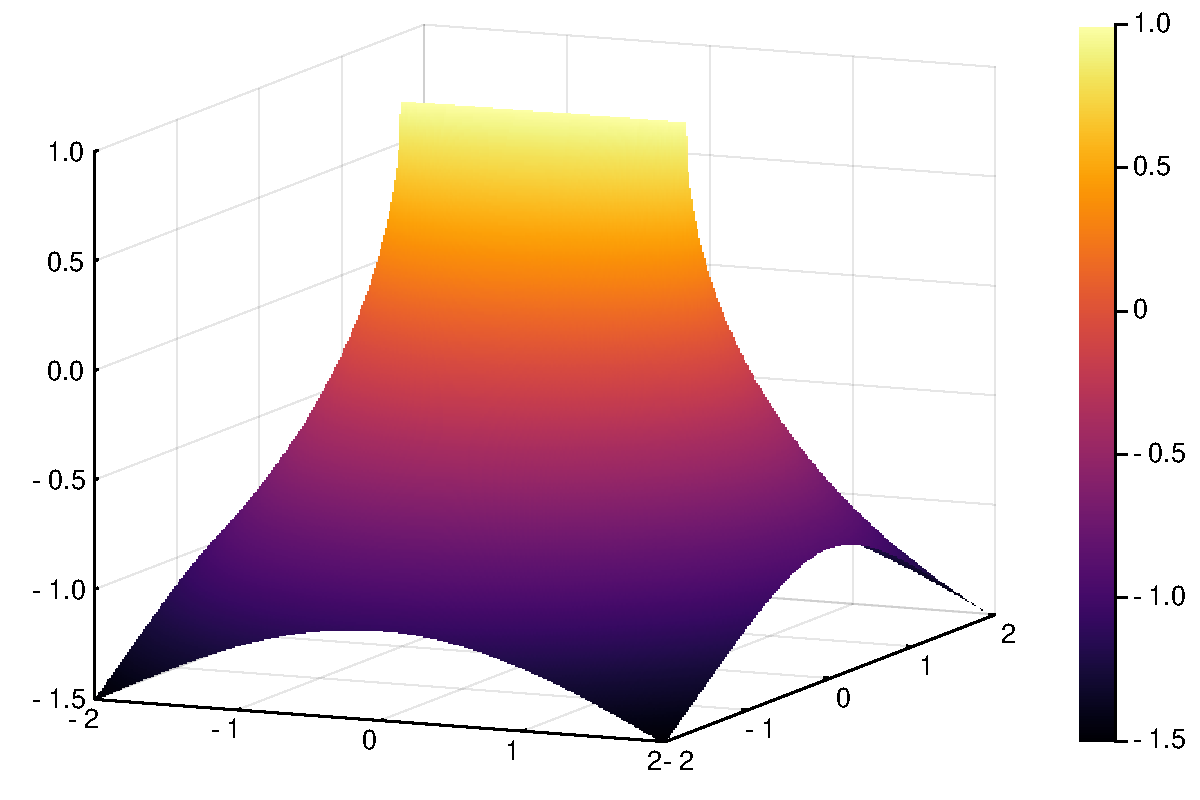
\includegraphics[width=\linewidth]{figures/Lecture19_5_1.pdf}

\subsection{Application: Potential arising from a point charge and a single plate}
Now imagine we put a point source at $x = 2$, and a metal plate on $[-1,1]$.  We know the potential on the plate must be constant, but we don't know what constant.  This is equivalent to the following problem (see e.g. \href{https://people.maths.ox.ac.uk/trefethen/chapman_hewett_trefethen.pdf}{[Chapman, Hewett \& Trefethen 2015]}):


\begin{align*}
v_{xx} + v_{yy} = 0 &\qqfor \hbox{$z$ off $[-1,1]$ and $2$}  \\
v(z) \sim \log |z - 2| + O(1) &\qqfor z \rightarrow 2 \\
v(z) \sim \log|z| + o(1) &\qqfor z \rightarrow \infty \\
v(x) = \kappa &\qqfor -1 < x < 1
\end{align*}
where $\kappa$ is an unknown constant.  We write the solution as

\[
v(z) = {1 \over \pi} \int_{-1}^1 u(t) \log|t-z| \dt + \log|z-2|
\]
for a to-be-determined $u$. On $-1 < x < 1$ this satisfies

\[
 {1 \over \pi} \int_{-1}^1 u(t) \log|t-x| \dt  = \kappa - \log(2-x)
\]
We can solve this equation explicitly. By differentiating we see that $u$ satisfies the following:

\[
\HH u(x) = f'(x) = {1 \over 2-x}
\]
We now use the inverse Hilbert formula to determine:

\[
u(x) = {1\over\sqrt{1-x^2}} \HH [{1 \over \diamond-2} \sqrt{1-\diamond^2}](x) + {D \over \sqrt{1-x^2}}
\]
Using the usual procedure of taking an obvious ansatz and subtracting off the singularities at poles and $\infty$ we find that:

\[
\CC[{\sqrt{1-\diamond^2} \over x -2}](z) = 
\underbrace{\sqrt{z-1} \sqrt{z+1} \over 2 \I (z-2)}_{\hbox{ansatz}} - \underbrace{\sqrt 3\over 2 \I (z-2)}_{\hbox{remove pole near $z=2$}} - \underbrace{{1 \over 2 \I}}_{\hbox{remove constant at $\infty$}}
\]
This implies that

\[
\HH[{1 \over\diamond-2} \sqrt{1-\diamond^2}](x) = -\I(C^+ + C^-)[{1 \over\diamond-2} \sqrt{1-\diamond^2}](x) = {\sqrt 3 \over x -2} + 1
\]
in other words, 

\[
u = {\sqrt{3} \over (x - 2) \sqrt{1-x^2}} + {D \over \sqrt{1-x^2}}
\]
We still need to determine $D$. This is chosen so that we tend to $\log |z|$ near $\infty$. In particular, we know that

\[
{1 \over \pi} \int_{-1}^1 \log|z-x| u(x) \dx \sim  {\int_{-1}^1 u(x) \dx \over \pi}  \log |z|
\]
so we need to choose $D$ so that $\int_{-1}^1 u(x) \dx = 0$ and only the $\log|z-2|$ singularity appears near $\infty$. We first note that 


\begin{align*}
C[{1 \over (\diamond - 2) \sqrt{1-\diamond^2}}](z) &= \underbrace{{\I \over 2 \sqrt{z-1} \sqrt{z+1} (z-2)}}_{\hbox{ansatz}} - \underbrace{{\I \over  2\sqrt{3} (z-2)}}_{\hbox{remove pole}} \\
& = -{\I \over 2 \sqrt{3} z} + O(z^{-2})
\end{align*}
near $\infty$. Since 

\[
Cw(z)  ={ \int_{-1}^1 w(x) \dx \over -2\pi \I z} + O(z^{-2})  
\]
we can  infer the integral from the Cauchy transform and find that

\[
\int_{-1}^1 {1 \over (x - 2) \sqrt{1-x^2}} \dx = -{ \pi \over \sqrt{3}}
\]
On the other hand,

\[
\int_{-1}^1 {\dx \over \sqrt{1-x^2}} = \pi
\]
Thus we require $D = 1$ and have the solution:

\[
u(x) = {\sqrt{3} \over (x - 2) \sqrt{1-x^2}} + {1 \over \sqrt{1-x^2}}
\]
\emph{Demonstration} 


\begin{lstlisting}
(*@\HLJLn{x}@*) (*@\HLJLoB{=}@*) (*@\HLJLnf{Fun}@*)(*@\HLJLp{()}@*)
(*@\HLJLn{u}@*) (*@\HLJLoB{=}@*) (*@\HLJLnf{sqrt}@*)(*@\HLJLp{(}@*)(*@\HLJLni{3}@*)(*@\HLJLp{)}@*)(*@\HLJLoB{/}@*)(*@\HLJLp{((}@*)(*@\HLJLn{x}@*)(*@\HLJLoB{-}@*)(*@\HLJLni{2}@*)(*@\HLJLp{)}@*)(*@\HLJLoB{*}@*)(*@\HLJLnf{sqrt}@*)(*@\HLJLp{(}@*)(*@\HLJLni{1}@*)(*@\HLJLoB{-}@*)(*@\HLJLn{x}@*)(*@\HLJLoB{{\textasciicircum}}@*)(*@\HLJLni{2}@*)(*@\HLJLp{))}@*) (*@\HLJLoB{+}@*) (*@\HLJLni{1}@*)(*@\HLJLoB{/}@*)(*@\HLJLnf{sqrt}@*)(*@\HLJLp{(}@*)(*@\HLJLni{1}@*)(*@\HLJLoB{-}@*)(*@\HLJLn{x}@*)(*@\HLJLoB{{\textasciicircum}}@*)(*@\HLJLni{2}@*)(*@\HLJLp{)}@*)
(*@\HLJLn{v}@*) (*@\HLJLoB{=}@*) (*@\HLJLn{z}@*) (*@\HLJLoB{->}@*) (*@\HLJLnf{logkernel}@*)(*@\HLJLp{(}@*)(*@\HLJLn{u}@*)(*@\HLJLp{,}@*) (*@\HLJLn{z}@*)(*@\HLJLp{)}@*) (*@\HLJLoB{+}@*) (*@\HLJLnf{log}@*)(*@\HLJLp{(}@*)(*@\HLJLnf{abs}@*)(*@\HLJLp{(}@*)(*@\HLJLn{z}@*)(*@\HLJLoB{-}@*)(*@\HLJLni{2}@*)(*@\HLJLp{))}@*)

(*@\HLJLn{xx}@*) (*@\HLJLoB{=}@*) (*@\HLJLn{yy}@*) (*@\HLJLoB{=}@*) (*@\HLJLoB{-}@*)(*@\HLJLni{4}@*)(*@\HLJLoB{:}@*)(*@\HLJLnfB{0.011}@*)(*@\HLJLoB{:}@*)(*@\HLJLni{4}@*)
(*@\HLJLn{V}@*) (*@\HLJLoB{=}@*) (*@\HLJLn{v}@*)(*@\HLJLoB{.}@*)(*@\HLJLp{(}@*)(*@\HLJLn{xx}@*)(*@\HLJLoB{{\textquotesingle}}@*) (*@\HLJLoB{.+}@*) (*@\HLJLn{im}@*)(*@\HLJLoB{*}@*)(*@\HLJLn{yy}@*)(*@\HLJLp{)}@*)

(*@\HLJLnf{contour}@*)(*@\HLJLp{(}@*)(*@\HLJLn{xx}@*)(*@\HLJLp{,}@*) (*@\HLJLn{yy}@*)(*@\HLJLp{,}@*) (*@\HLJLn{V}@*)(*@\HLJLp{)}@*)
(*@\HLJLnf{plot!}@*)(*@\HLJLp{(}@*)(*@\HLJLnf{domain}@*)(*@\HLJLp{(}@*)(*@\HLJLn{x}@*)(*@\HLJLp{);}@*) (*@\HLJLn{color}@*)(*@\HLJLoB{=:}@*)(*@\HLJLn{black}@*)(*@\HLJLp{,}@*) (*@\HLJLn{legend}@*)(*@\HLJLoB{=}@*)(*@\HLJLkc{false}@*)(*@\HLJLp{)}@*)
\end{lstlisting}

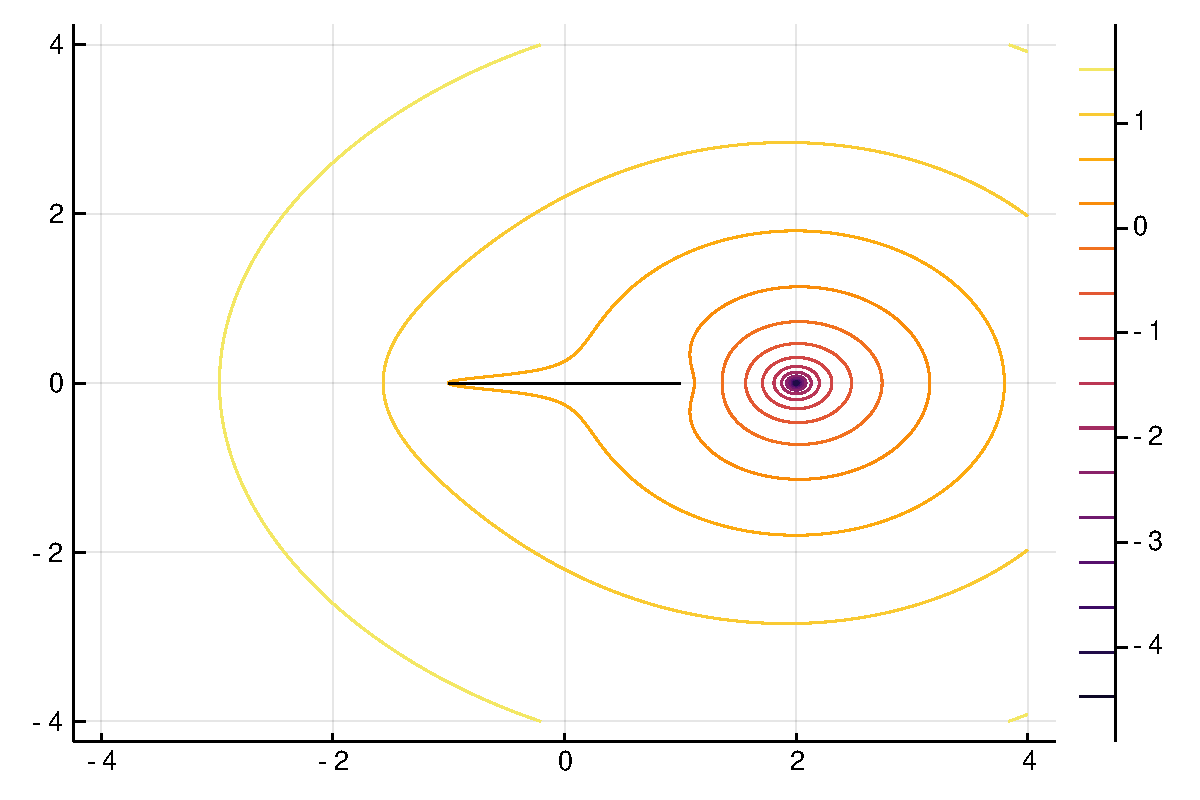
\includegraphics[width=\linewidth]{figures/Lecture19_6_1.pdf}

We can compute $\kappa$ numerically:


\begin{lstlisting}
(*@\HLJLnf{v}@*)(*@\HLJLp{(}@*)(*@\HLJLnfB{0.2}@*)(*@\HLJLp{)}@*)
\end{lstlisting}

\begin{lstlisting}
0.6238107163648714
\end{lstlisting}



\end{document}
